%!LW recipe=pdflatex ➞ bibtex ➞ pdflatex`×2

\documentclass[twocolumn]{article}

\usepackage[backend=bibtex]{biblatex} 
% \usepackage{kpfonts} 
\usepackage[margin=2cm]{geometry} 
\usepackage{hyperref} 
\usepackage{siunitx} 
\usepackage{graphicx} 
\usepackage[super]{nth} 
\usepackage{tabularx} 
\usepackage{ltablex} 
\usepackage{longtable} 
\usepackage{subcaption} 
\usepackage{booktabs}
\usepackage{multirow}

\addbibresource{../references.bib} 

\title{An Investigation Into Methods for the Detection of \\Malicious Software Using Techniques from Machine Learning} 

\author{ Henry Williams\textsuperscript{1} }

\date{\footnotesize\textsuperscript{\textbf{1}}School of Engineering and Informatics, The University of Sussex}

\begin{document}

\maketitle 

\vspace{1.5em}

{
    \centering 
    {\large \textbf{Abstract}}

    \vspace{1em}

    In this report, we outline our plan for our investigation into approaches for the detection of malware which utilise techniques from machine learning. Our investigation will rigorously evaluate these approaches on a custom dataset of windows executables. In addition to this, we will also investigate any potential means by which we can improve these approaches, and how effectively the models we investigate handle obfuscation.  
}

\section{Introduction}

Malicious software, otherwise known as malware, are a form of computer software which intentionally perform unwanted or harmful actions on a system, without the users consent~\cite{kramer_general_2010}. Security researchers consider these programs to be one of the most widespread risks faced by both individuals and organisations. In order to mitigate these risks, a number of systems to detect and flag malware before it can infect a system have been proposed~\cite{bitdefender2025official,avast2025official,malwarebytes2025official}. However, these rely on a database of known malicious software, rendering them ineffective against new malware. Furthermore, the developers of these programs will typically employ techniques to confuse these scanners, known as obfuscation~\cite{you2010obfuscation}, further reducing their efficacy. 

Machine learning enables for more accurate, and robust detection of harmful programs, by learning characteristics indicative of a programs' ill intent. This greatly reduces the risk posed by such programs~\cite{huda_hybrid-multi_2018,li_dmalnet_2022,karbab_maldozer_2018,vinayakumar_robust_2019}, and has been an active area of computer security research. 

Our investigation will provide a rigorous evaluation of various approaches utilising machine learning to discriminate between both malicious, and non-malicious software, which we refer to as benign software throughout this report. Our experiments will take place on a custom dataset containing benign, and malicious executables in the Windows Portable Executable file format, and we will test both static and dynamic approaches. 

\section{Background}

\subsection{Malware}

% What is malware? 
Malware are software which perform unwanted or harmful actions on a host system. Security researchers often classify these programs into various categories based on their behaviour which are explored in Section~\ref{sec:malware-types}. 

As we become increasingly reliant on digital infrastructure in our daily lives, mitigating the risk posed by malware is of the utmost importance. For example, in 2017, ransomware known as WannaCry begun spreading throughout the internet, infecting an estimated 300,000 systems~\cite{akbanov2019wannacry}. One of the most prominent victims of this attack was the National Health Service, who were unable to access patient information, and make use of vital medical equipment for its duration~\cite{nao2017wannacry}. Furthermore, it is estimated that the damages to systems infected by WannaCry costed the global economy \$4 Billion~\cite{akbanov2019wannacry}. This shows not only the potential financial impact of these programs, but the potential human cost as well, and why preventing such an attack is so important. 

\subsection{Windows Portable Executable File Format}\label{sec:pe}

\begin{figure}
    \centering 
    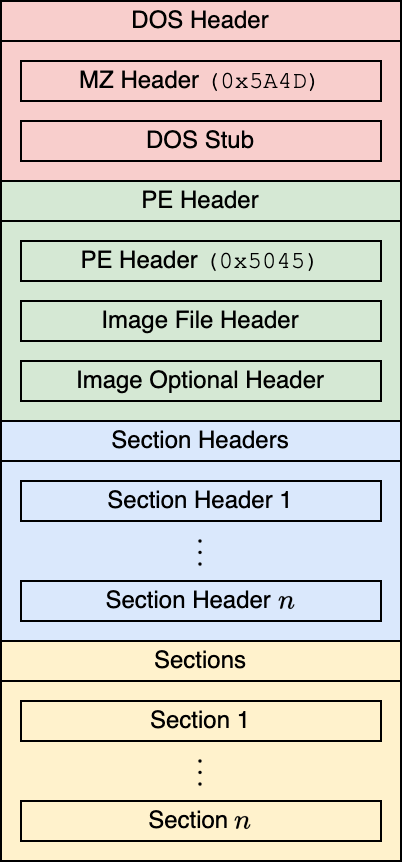
\includegraphics[width=0.3\textwidth]{../assets/pe.png}
    \caption{A high level overview of the windows portable executable file format.}
    \label{fig:pe}
\end{figure}

Executables targeting the Windows operating system are written in the Portable Executable (PE) file format. These files are often not written by developers themselves as they require expert knowledge of low level programming, and instead are generated by a compiler. A high level overview of this file format is shown in Figure~\ref{fig:pe}, and it has been used since Windows 95, making it incredibly widespread throughout the internet. 

The file begins with a DOS (Disk Operating System) header for compatibility reasons~\cite{karl-bridge-microsoft_pe_2024}, followed by the PE header, containing information necessary for its execution. This includes the number of sections and symbols, and the instruction set used by the program. The section headers contain further metadata about the sections which comprise the program, and reference their location in memory. It also stores a pointer to a table referencing any external functions used by the program, such as the Windows API\@, and other dynamically linked objects, known as DLLs~\cite{deland-han_dynamic_2024}. 


\subsection{Types of Malware}\label{sec:malware-types}

One of the earliest forms of malware, known as a \emph{virus} is a self replicating program which modifies other executables to infect new targets. In order to spread, they rely on the user unknowingly sharing an infected file to a new host. 

Unlike a virus, \emph{Worms} propagate throughout a network without the need for user interaction, and will often make use of software exploits to infect new targets. They are considered to be extremely dangerous, as they can rapidly spread throughout a network.

\emph{Trojan Horses} present themselves as legitimate software in an attempt to trick users into infecting their devices. This is one of the most widespread forms of malware in the current era, as it is far easier to trick someone into downloading software than it is to develop sophisticated software exploits. 

\emph{Spyware} refers to a category of malware which exfiltrate private information, such as password, cookies and internet traffic from the host machine, likely to be resold or used to further compromise the victim. 

\emph{Root Kits} are installed into the operating system, unlike other malware which are installed to user space. This provides the program with the highest possible level of privilege, meaning it has direct access to operating system functionality, hardware, and external peripherals. As a result of this, this forms of malware is extremely powerful, and can be extremely difficult to detect once infected. 

\emph{Ransomware} refer to malware which hold a system captive, typically by encrypting the files stored by the host, until a ransom is paid. 

\emph{Bots} are a form of malware which enable an attacker remote control of a host system. These are typically part of a larger network of infected systems, known as a \emph{botnet}, which are often used as part of distributed denial-of-service attacks. 

It is worth noting that these categories are not mutually exclusive, and malware often exists in more than one class at once. 

\subsection{Detection}

Early attempts at malware detection rely upon the file signatures of programs given by a cryptographic hash function. This signature of an unknown program is compared against a database containing the signatures of malware, and if the hash is present within the database, then we know the program is malicious, and can be flagged as such. 

However, if the program is not present within the database, it will always be treated as benign.  This means that if a malware is yet to be seen within the database, it will be allowed to execute, infecting the hosts. Malware authors exploit this by making small changes to their software, leading to an entirely new file signature, thus tricking the detection software. 

More sophisticated systems fall into one of two categories, \emph{static}, and \emph{dynamic}. Static detection services determine the intent of a program, without executing it, typically making them faster, at the cost of being less accurate, due to their heavily obfuscated nature. For example, they may consider metadata found within a program, which includes external subroutines, and static strings found within the program. 

Dynamic Detection observes the execution of a program. This is often more powerful than static approaches, as it considers a programs' behaviour rather than its structure. However, in order to run these programs safely, an isolated environment such as a virtual machine is needed. Some forms of malware also make use of anti-analysis features, which checks the execution environment, and determines if it is inside a virtual machine before executing its malicious portion to trick dynamic analysis tools.  

\subsubsection{Machine Learning}

Machine Learning for malware detection has been an active area of research~\cite{merabet_survey_2019,tayyab_survey_2022}, as it enables software to learn common features of malware which other software may not be able to detect. This enables more accurate and resilient classifiers, and in this section, we outline a handful of approaches seen in our research. 

An executable program is merely a series of instructions and data, which are interpreted by the host system. These instructions are expressed in a language known as machine code which largely follows the pattern of an instruction, known as an opcode refering to the byte used to denote the operation, followed by some operands. The approach outlined in~\cite{azmoodeh2019robust} describes a classifier which makes use of n-grams, graph learning, and deep eigenspace learning to train their model, achieving 99\% accuracy. In this opcode n-gram graph, edges between verticies in this graph are given by the probability of the proceeding instruction being another opcode. The authors then use a Convolutional Neural Network to learn the classification based on the first and second eigenvalues of the adjacency matrices previously generated.

However, their data set was extremely imbalanced, with approximately 1000 benign samples, and only 100 malicious samples. Furthermore, the investigation performed in~\cite{raff_investigation_2018} suggests these features are not sufficient, due to the lack of meaningful information. 

Other textual features can also be extracted from executables, such as the strings stored used by the program. These can also provide a lot of information about the nature of the program which can be used to learn classification, as was performed in~\cite{tian2009strings}, achieving 97\% detection accuracy. This approach utilises the WEKA classification interface~\cite{frank2016weka}. 

The header of an executable also provides useful information, which is used by the authors of~\cite{shafiq2009pe}, to achieve an average detection accuracy of 90\%. Their approach makes use of textual features found in the headers of the executable, which are preprocessed and used to train linear classification algorithms, such as Naive Bayes. 

\begin{figure}
    \centering 
    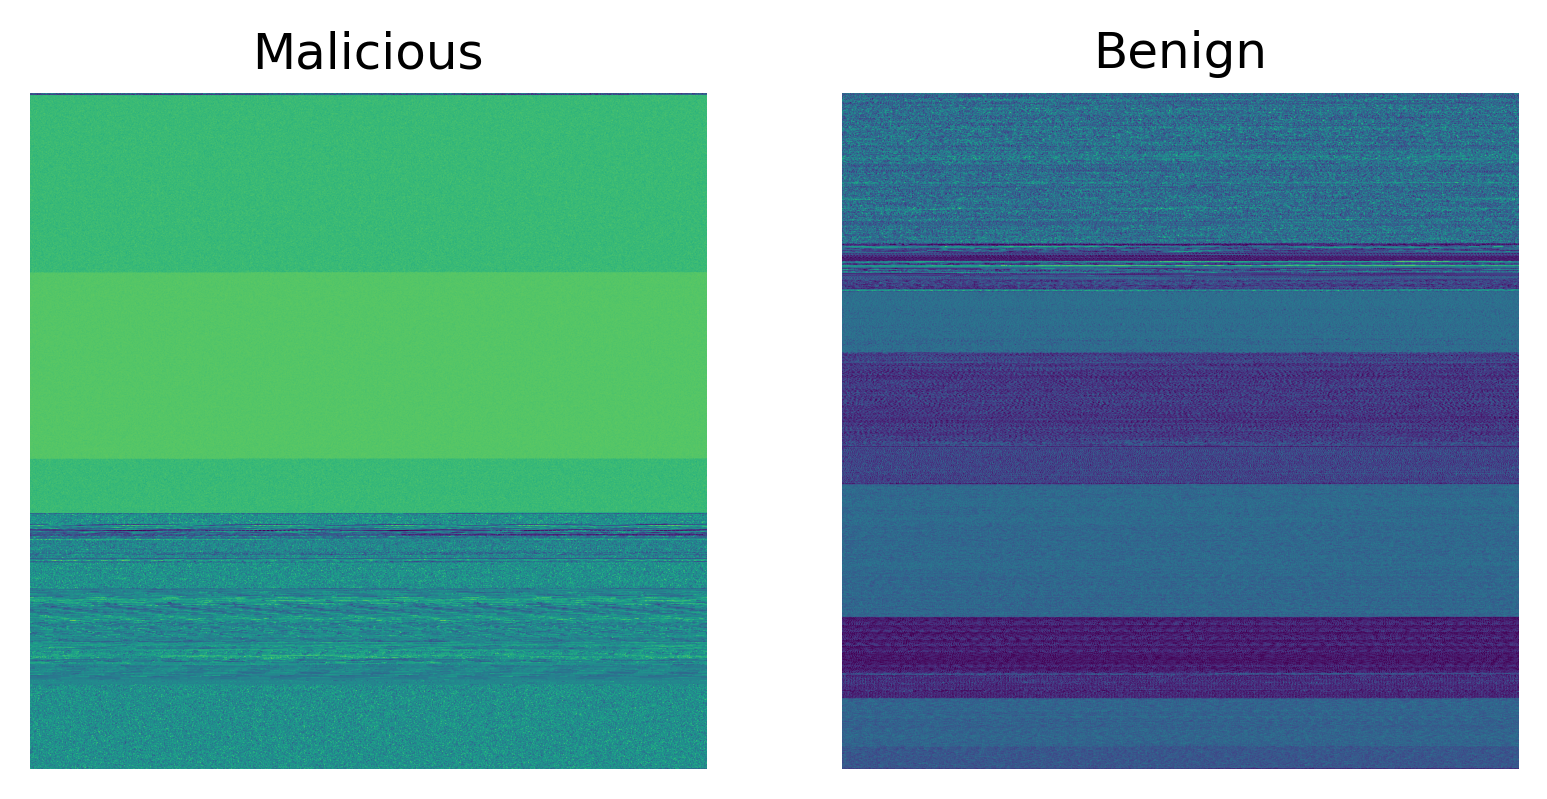
\includegraphics[width=0.4\textwidth]{../assets/mal-ben-img.png}
    \caption{Malware and benign programs represented as images}\label{fig:mal-ben-img}
\end{figure}

Another approach for static malware analysis is to represent the programs as images (Figure~\ref{fig:mal-ben-img}) either for further augmentation, or trained on directly using a Convolutional Neural Network (CNN). Approaches using this technique seem to vary in terms of efficacy, for example, in~\cite{nataraj2011malware}, the authors were able to achieve 98\% classification accuracy, whereas the authors of~\cite{su2018lightweight} were only able to achieve 94\%. This is likely due to the authors requirements of building a lightweight model for detection.  

Dynamic analysis is often significantly more powerful than static analysis. For example, the authors of~\cite{li_dmalnet_2022} make use of graph learning based on API calls, and their shared arguments, to develop a highly accurate detector which is resilient to most forms of obfuscation. Other approaches make use of API call sequences~\cite{han_maldae_2019}, file system modifications~\cite{pektas_classification_2017}, and network communications~\cite{schwenk2011adaptive}.

An approach we have not yet seen in our research is Attention based models~\cite{vaswani2023attentionneed}, which learn the relative importance of components in a sequence. These are widely used in sequence modelling, and natural language processing, and are extremely powerful. As part of our investigation, we plan on developing our own attention based model for malware detection, and comparing it to other approaches. 

\subsection{Obfuscation}\label{sec:malware-obfuscation}

\begin{figure*}
    \begin{subfigure}[c]{0.5\textwidth}
        \centering
        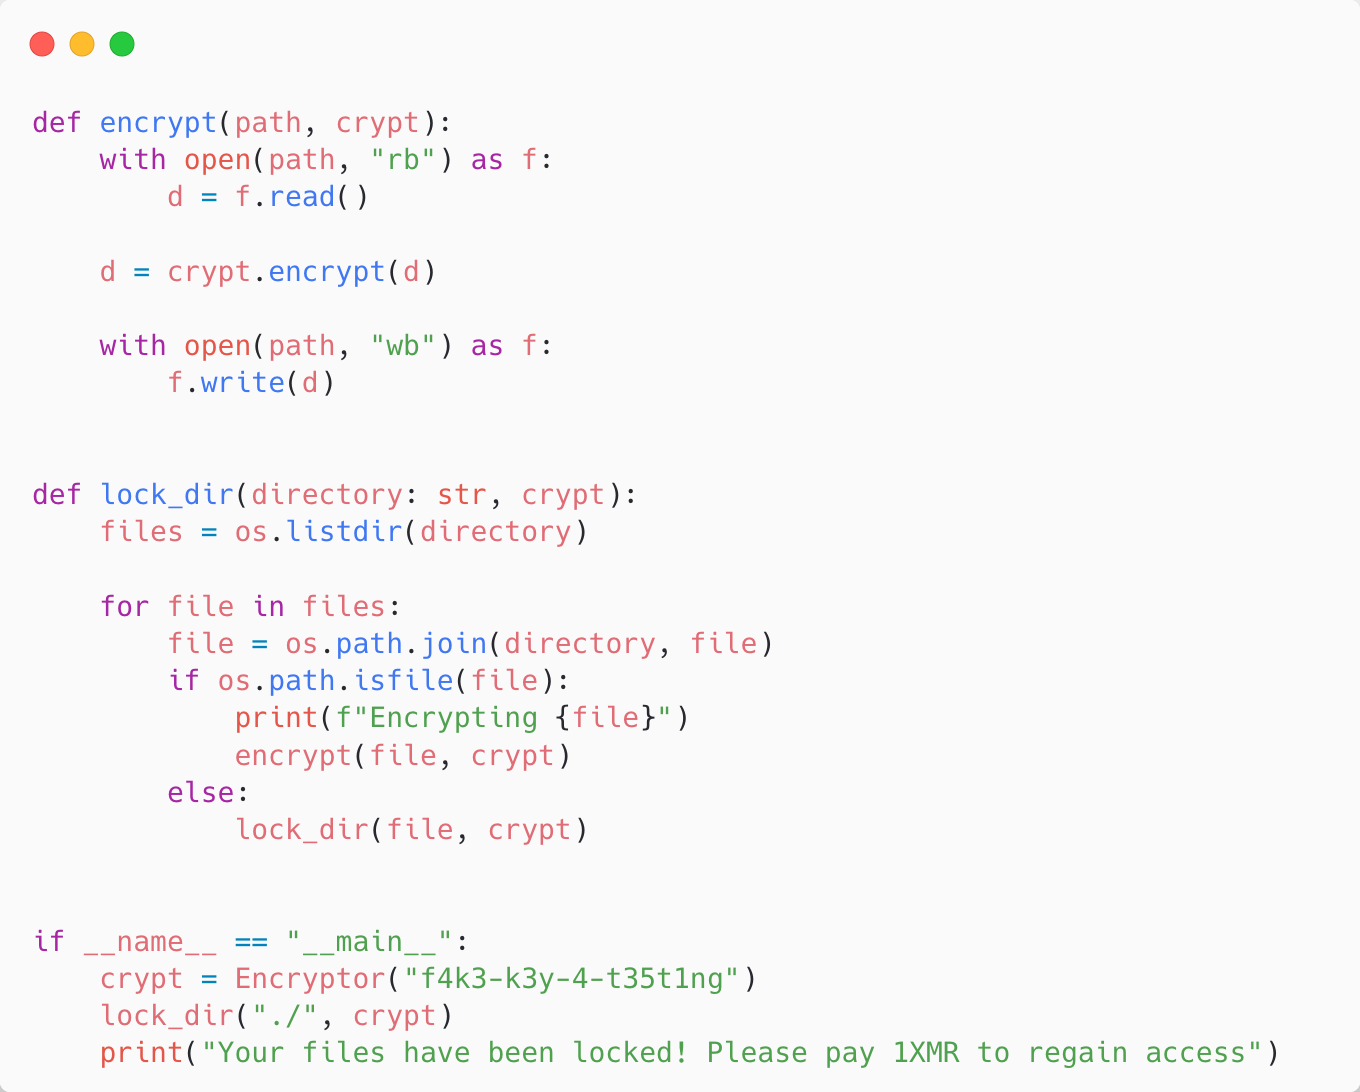
\includegraphics[width=0.6\textwidth]{../assets/malware-unobf.png}
        \caption{A simple piece of malware.} 
        \label{sfig:malware}
    \end{subfigure}
    \begin{subfigure}[c]{0.5\textwidth}
        \centering
        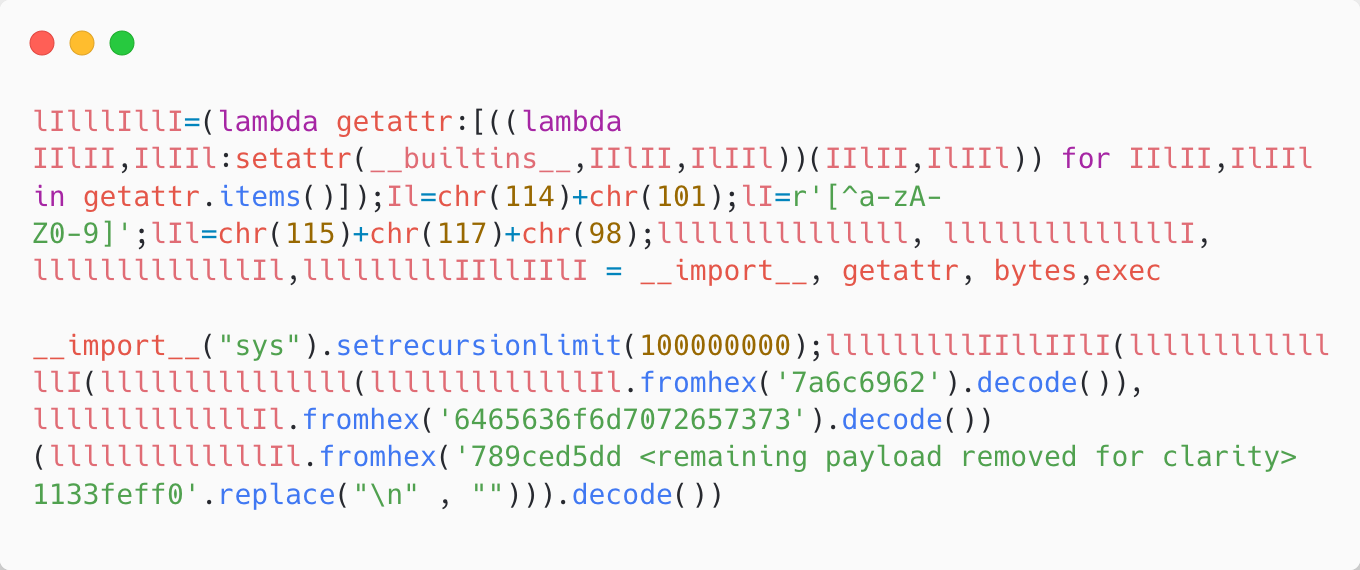
\includegraphics[width=0.6\textwidth]{../assets/malware-obfs.png} 
        \caption{The same program shown in~\ref{sfig:malware}, but obfuscated.}
    \end{subfigure}
    \caption{An example of how a piece of malware may be obfuscated.}
    \label{fig:obfs}
\end{figure*}

Obfuscation, shown in Figure~\ref{fig:obfs}, refers to a set of techniques which make understanding a piece of software more challenging, while still performing the same operations. 

\subsubsection{Encrypted Malware}

This form of obfuscation employs encryption algorithms, to hide its  purpose. 

Malware that employ this form of obfuscation are typically composed to two parts, the encrypted main body and decryptor~\cite{yaacoubi2019encrypted}. Upon running the program, the decryptor recovers the main body, which is then executed. This bypasses signature based detection, as each new infection uses a different key. However, the decryptor portion remains constant across instances.

Oligomorphic malware extends upon this idea, by modifying the decryptor portion of the program to further confuse detection software. This enables to evade detection far more effectively than encryption alone~\cite{you2010obfuscation}. 

\subsubsection{Polymorphic Code}

Polymorphic code refers to a program which modifies its own instructions, but performs the same operations. Malware utilising this form of obfuscation mutate their structure upon each new infection. The mutations made to the program could include randomly re-assigning registers, inserting dead code and data, among other more advanced techniques. This form of obfuscation is incredibly powerful, as existing detection engines would struggle to find patterns between instances of polymorphic code, making detection extremely difficult. 

\subsubsection{Dead Code Insertion}

\begin{figure}
    \centering 
    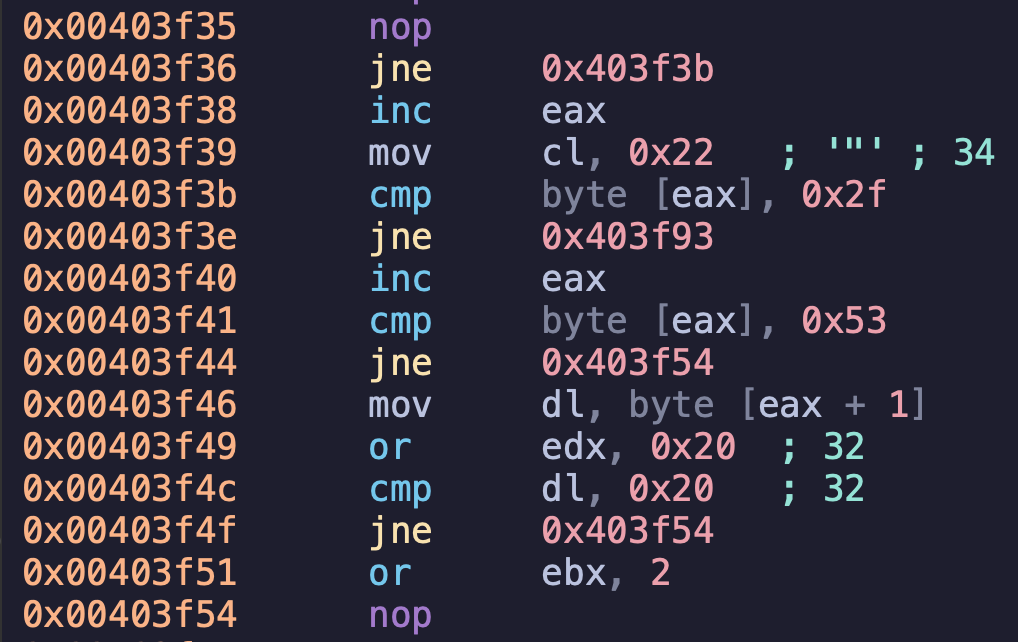
\includegraphics[width=0.4\textwidth]{../assets/dead-code.png}
    \caption{Dead code insertion within a piece of malware, written as ``nop''}
    \label{fig:dead-code}
\end{figure}

One of the less sophisticated forms of obfuscation is to simply insert instructions which have no purpose in the program. This could include no-operations (Figure~\ref{fig:dead-code}), which tell the CPU to do nothing, or performing useless operations, such as modifying an unused register. 

\section{Aims}

The aims of this project are as follows: 

Firstly, we aim to curate a large, comprehensive dataset containing a diverse collection of programs. The programs found in this dataset, both malicious and benign, should exhibit a diverse range of characteristics  relating to their functionality. For example, if a majority of our malicious samples are console applications, and our benign samples consist of programs with a graphical user interface, then the models we test will simply learn to classify based on the presence of a user interface. 

Next, we aim to perform a rigorous evaluation of machine learning techniques for detection, trained on our dataset. We will investigate the overall accuracy of these models, in addition to their robustness to obfuscation techniques. This will require the development of an experimental framework to ensure consistency between the approaches we test.

Finally, we aim to investigate any potential avenues for new ideas and approaches that could increase the efficacy of the models we test in our experiments. This includes attention based models, as we are yet to see much research into this area. 

Further work in this field could investigate how well the models we test can be applied to other domains, such as on different operating systems such as Unix based hosts. 

\section{Project Plan}

\begin{figure*}
    \centering 
    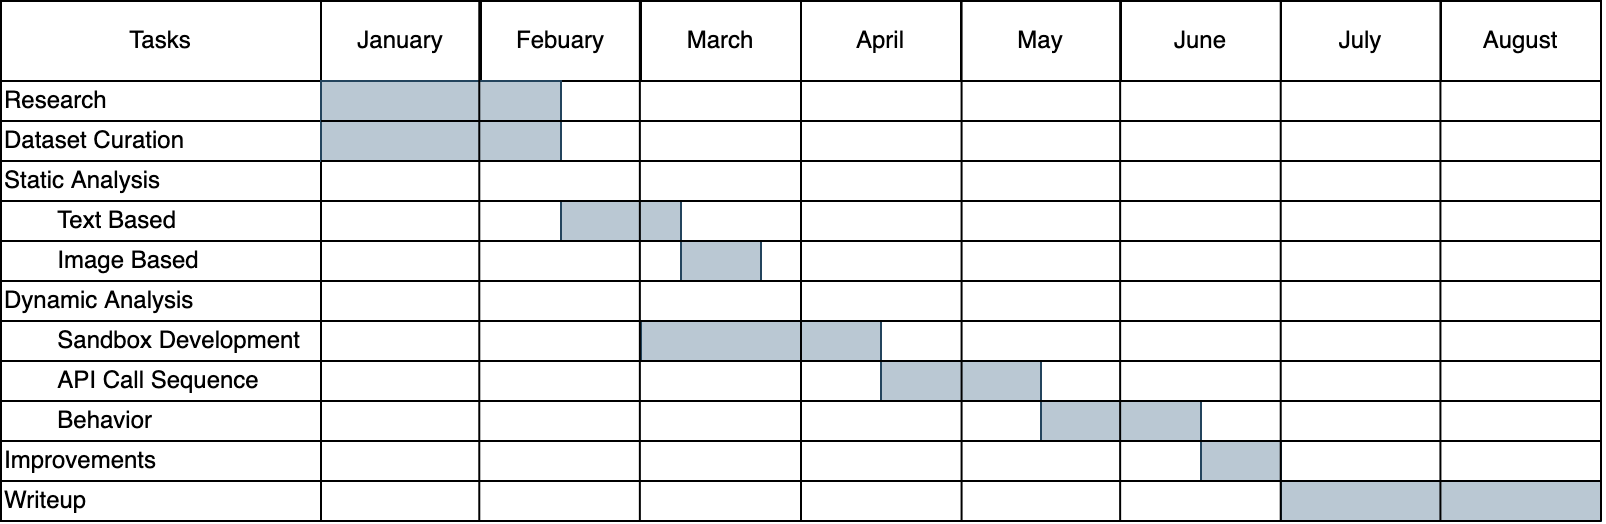
\includegraphics[width=0.8\textwidth]{../assets/gantt-chart.png}
    \caption{Gantt Chart outlining the expected timeline of our investigation.}
    \label{fig:gantt-chart}
\end{figure*}

In figure~\ref{fig:gantt-chart}, we outline the expected timeline for our investigation. We begin by firstly determining which approaches we will test as part of our investigation. In parallel to this, we will also be curating the dataset we use in our experiments. This has been allocated a significant portion of time in order to ensure the dataset is representative of software used by in everyday operation, and the forms of malware that may be encountered. 

Upon deciding the approaches we plan to investigate, and the completion of our dataset, we will investigate static approaches to malware detection. We have separated this into two sub tasks, however, this may change over the course of our research into other potential approaches. We plan on completing our experiments in this area by mid march in order to have enough time to begin development of the sandboxing framework necessary to perform dynamic analysis. 

We plan on using the Panda-RE framework~\cite{gavitt2015panda} for our sandbox, as it enables researchers to hook into certain operating system functionality, and record the executions of programs on the host. It can also allow us to modify certain operating system functionality, such as internal APIs in order to defeat anti-analysis systems often found in malware. In our limited experimentation so far, we have been unable to get this service working, so we have allocated additional time for this task. If we are unable to get it working in a reasonable time frame however, other platforms such as CAPE~\cite{capesandbox}, and Noriben~\cite{baskin_ruriknoriben_2025} offer similar functionality. 

Once a framework for performing dynamic analysis is achieved, we will begin our investigation into dynamic detection methods. We expect this to take longer than the static analysis investigation, and as such, we have allocated additional time. 

Should we find any potential avenues for improving upon the approaches we investigate as part of our research, we will spend 2 weeks developing and evaluating it. One such avenue we plan on investigating are attention based mechanisms, as we are yet to see much research into these models for this purpose.

Finally, we have allocated at least a month to complete the write up of our investigation.

\subsection{Ethical Considerations}

In this investigation, we will be using a dataset containing malicious software. Because of this, there are several ethical considerations that we must consider to ensure that our work maintains scientific and academic integrity. 

The most significant consideration relates to ensuring personal and university infrastructure are not effected by the potentially dangerous software throughout our investigation. We will ensure that the execution of software within our dataset will only occur within a safe, isolated environment. To mitigate the risk of accidentally running a malicious program, we have marked all samples as non-executable, meaning that in order to run them, the user must explicitly mark them as executable before they can be executed.

It is worth noting however, that it is possible to escape these isolated environments~\cite{beer2022forcedentry}. This form of exploit is known as a sandbox escape. However, due to the complexity of such exploits, they are extremely rare, and often only available to Advanced Persistent Threats, such as nation state hackers. 

Furthermore, the benign samples found within our dataset will need to be representative of software used in day-to-day operations. These programs are often copyrighted, so we must ensure they are not distributed with unauthorised users to prevent any legal issues. We have stored our dataset on a external drive, which will not be shared with anyone outside of the project. 

\section{Data}

Existing datasets for this problem, such as the Elastic Malware Benchmark for Empowering Researchers (EMBER)~\cite{anderson2018ember}, consist of features extracted from executables, limiting the applications for which it can be used. Furthermore, the executables from which these features are derived are unavailable due to licensing issues~\cite{harang2020sorel20m}. As our investigation will test a variety of different approaches, which all make use of different features, we require the executables themselves to extract the required information. Other datasets we have looked at have similar issues regarding licensing, or are comprised of executables for other operating~\cite{freitas2022malnetlargescaleimagedatabase}. It is for these reasons that we plan on building our own custom dataset. 

Our dataset will consist of executables in the windows PE file format. Malicious samples are collected from the virusshare database~\cite{noauthor_virussharecom_nodate} which contains over 90 million samples seen in the wild. It also provides detection information from a number of sources including its classification. We have downloaded over 5000 malware samples from this database, and we can always download more if it is deemed necessary.  

Finding a similarly sized collection of benign software could raise some issues however. Other research in this field makes use of websites offering free, portable software such as~\cite{noauthor_portableappscom_nodate} and~\cite{noauthor_latest_nodate}. We have also investigated package managers such as chocolatey~\cite{noauthor_chocolatey_nodate} and winget~\cite{noauthor_microsoftwinget-cli_2025}, which provide large repositories of verified benign software that can be used freely. We have also considered the possibility of synthetic data, and scraping platforms such as GitHub should the approaches we outline above prove insufficient. In this case, synthetic data could be generated using large language models.

As malware often hides itself within a legitimate program, this could raise issues when it comes to reliable detection. To remedy this, we plan on performing pairwise similarity analysis, using the Locality Sensitive Hashing algorithm~\cite{leskovec2020mining}, to locate and remove benign samples where a similar malicious variant exists. 

We will also investigate the use of augmentation techniques to modify our data. This will include the obfuscation of benign executables to make the problem more challenging. This could provide insights into how well models deal with obfuscation. Furthermore, we could categorise our dataset based the classes we discuss in Section~\ref{sec:malware-types} in order to see which models are best on certain forms of malicious software, and if any types of malware are generally easier to detect overall. 

\section{Conclusion}

In this report, we have outlined our plan for an investigation into malware detection using techniques from deep learning. We have outlined why detection of malware is important, the different forms of malware seen in the wild, the techniques employed by malware authors to make detection more difficult, and existing attempts at malware detection. We introduce our plan for the project, and any potential ethical issues we must consider as part of our investigation. Finally, we discuss the data we plan on using as part of our investigation.  

\printbibliography
\end{document}
